
\chapter{The Eletronics} \label{chap:electronics}

In order for the aircraft to fly and navigate autonomously, onboard electronics are required, for both actuation, power source, and navigation. Some of the used electronics were already available, and were chosen for this reason.
	
\section{Propulsion}

Due to the familiarity and availability, the Mikrokopter Mk3538 Motor was chosen, paired with E-Max Simon 60A escs.

Experimental curves for the motor are available at Mikrokopter's website, and the relevant ones are reproduced on Figure \ref{fig:motorcurves}. Each motor should give, on 16 V, around 1.9 kg of static thrust when paired to 12 inches propellers, up to 2.5 kg on 15 inches, while drawing 35 A, or about 560 W.

\begin{figure}[H]
\centering
  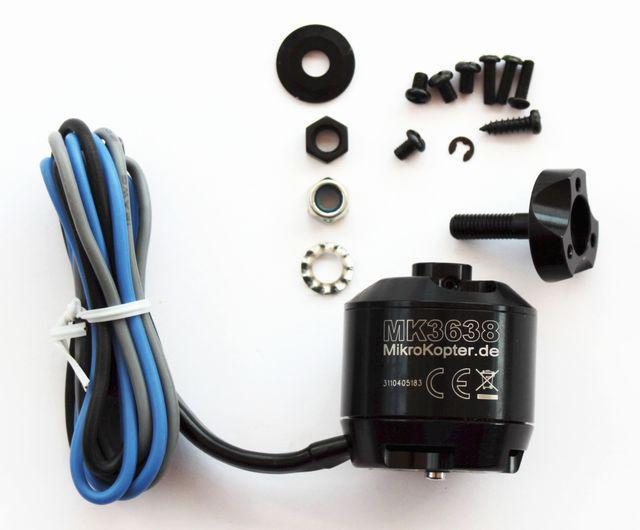
\includegraphics[width=0.8\linewidth]{figs/mk3638.jpg}
  \caption{Mikrokopter MK3638 Brushless Motor.}
  \label{fig:yaw_loop}
\end{figure}

\begin{figure}[h]
  \centering
  \begin{subfigure}{.8\textwidth}
    \centering
    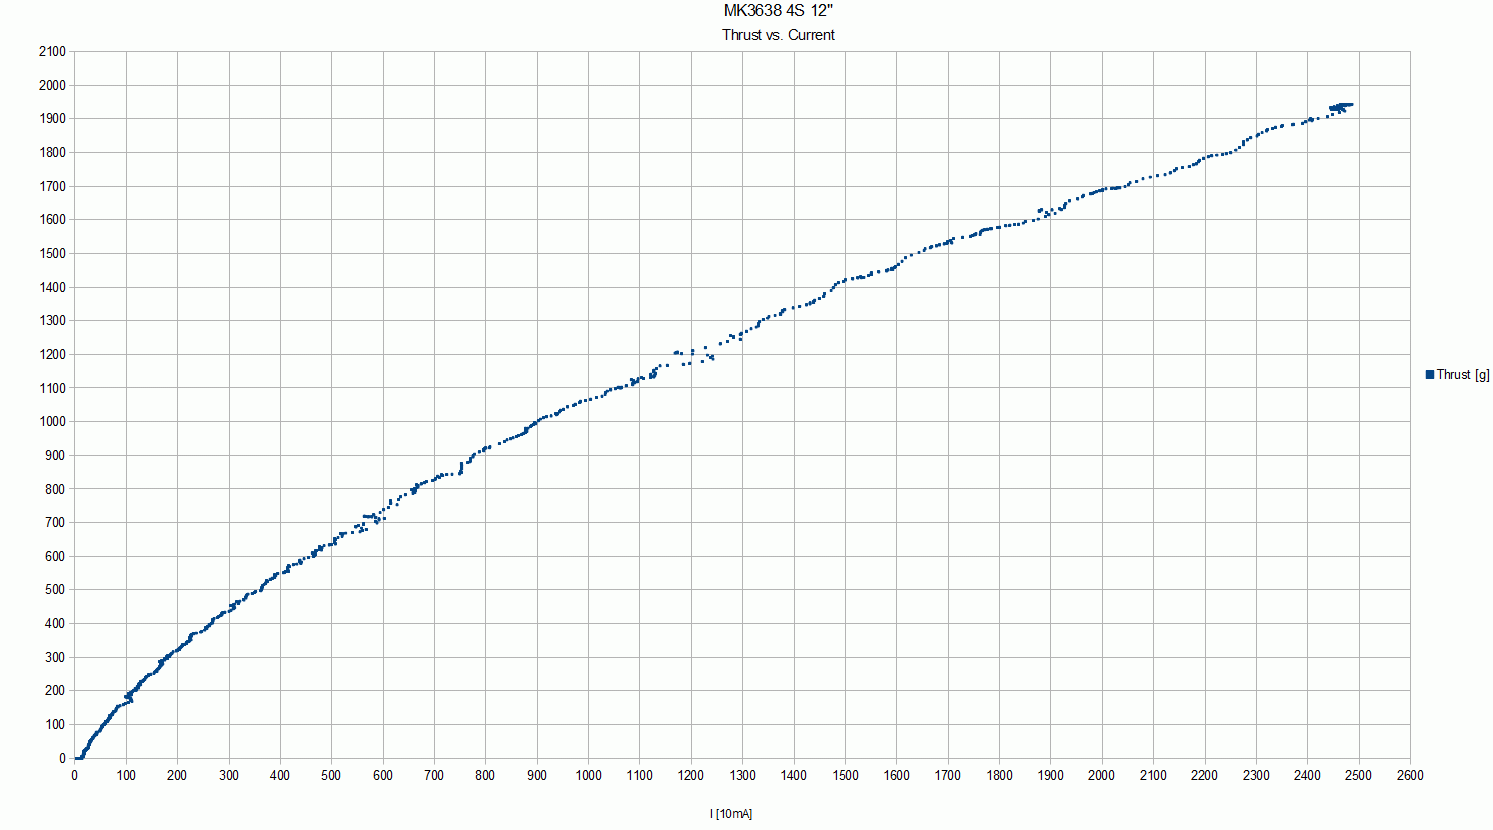
\includegraphics[width=\linewidth]{figs/curve12.png}
  
  \end{subfigure}%
  
  \begin{subfigure}{.8\textwidth}
    \centering
    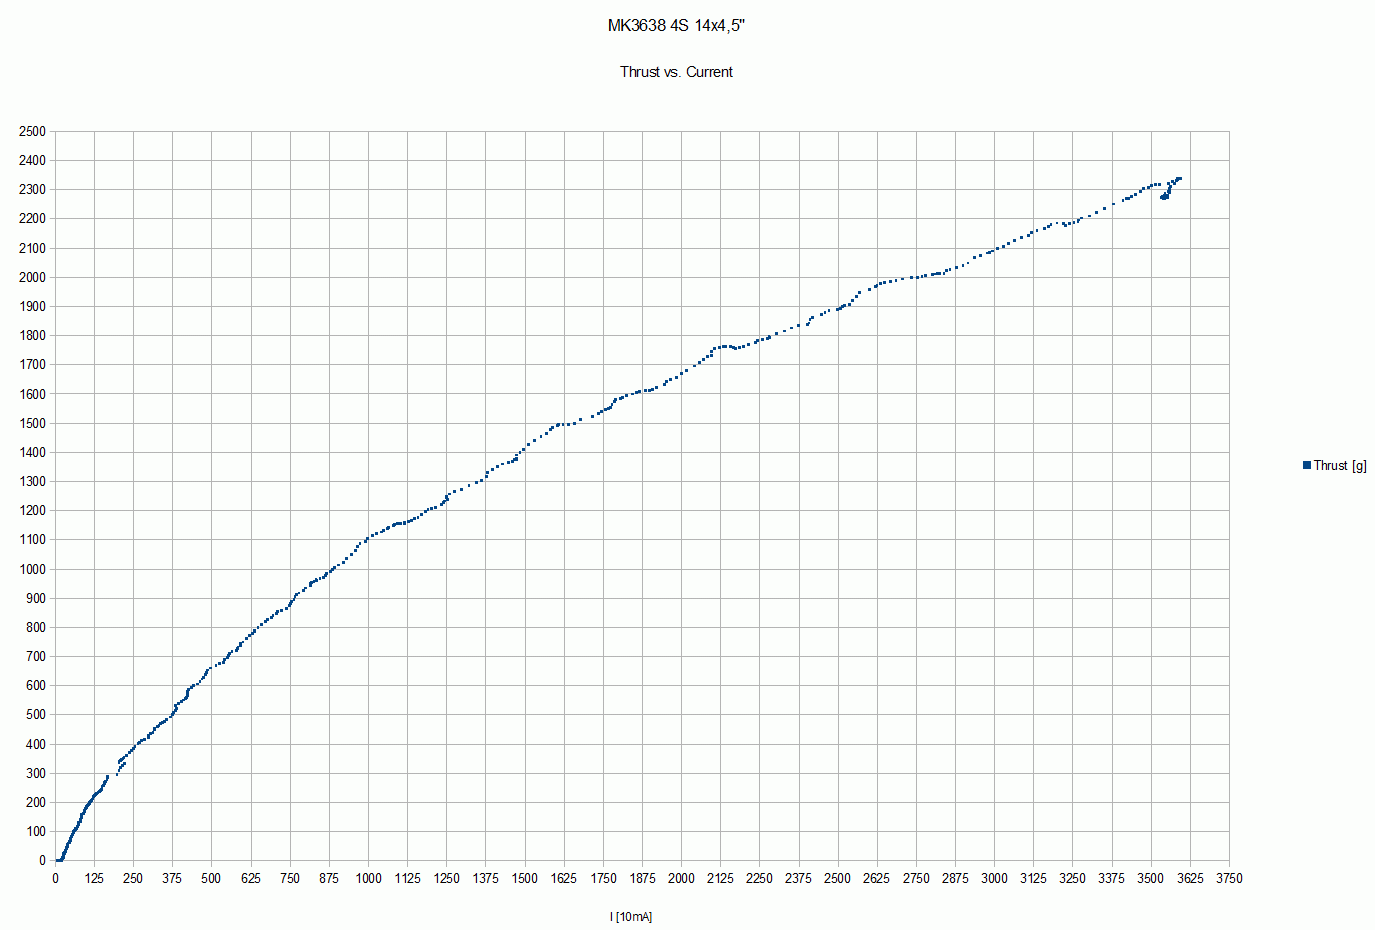
\includegraphics[width=\linewidth]{figs/curve15.png}

  \end{subfigure}
  \caption{Motor curves with 12 and 15 inches propellers.}
  \label{fig:motorcurves}
\end{figure}


As the airplane is aimed to weigh around 3 kg, each motor needs to pull at least 1500g for hovering, leaving a maneuvering margin of around 1 kg for each motor.

\section{Batteries}

As each motor can draw up to 35 A, the battery should be able to provide up to 70 A without issues.
The Batteries chosen are also the ones already in use by the company, Multistars 10000 mAh 10C, which, at 10 C rating, are able to sustain a constant draw of up to 100 A. 

Each weigh approximately 750 g and measures XXxYYxZZ mm.
\todo{medir}

\begin{figure}[H]
\centering
  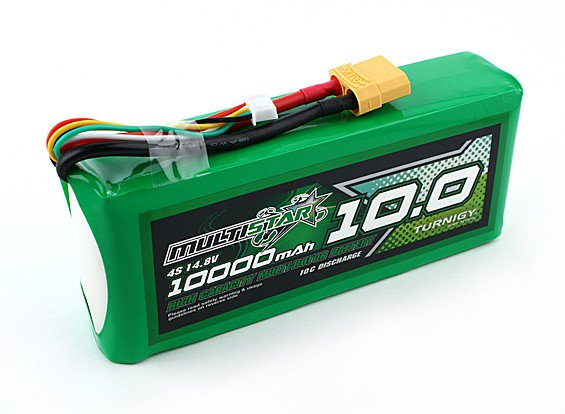
\includegraphics[width=0.8\linewidth]{figs/battery.jpg}
  \caption{Multistar 4s 10000 mAh Lithium Polymer battery.}
  \label{fig:yaw_loop}
\end{figure}


\section{The Servos and Control Surfaces}

The control surfaces must be slightly larger than usual for a flying wing, as on a tail-sitter a reasonable amount of air must be deflected on hover situation, while on most wings a steady airflow is assumed. It's suggested to have control surfaces taking up to 30\% of the chord of the wings. Since they are easily swappable, it was decided to start with smaller ones, with a 10 cm chord, and replace them if necessary.


The servos chosen were standard servos Savox SV-0220, linked to the elevon horns with a stiff wire.

\begin{figure}[H]
\centering
  \includegraphics[width=0.8\linewidth]{figs/serv.jpg}
  \caption{Savox SV-0220 servo.}
  \label{fig:yaw_loop}
\end{figure}

\section{The Flight Controller}

The multirotor had a huge boom last 10 years. In 2009 the first hobby-grade flight controller for multicopters was born, Rolf "KaptainKuk" Bakke's "KK board". Using a simple AVR controller and three gyroscopes, the board could control angular speed on three axis, enabling pilots to control the multirotors. It was programmed in AVR assembly and had individual PID controllers for each axis.
%
Shortly after, Alexinparis noticed the gyros on the Wii Motion + controller, and MultiWii was born. This project grew to support a variety of sensors and boards, and had an active development community, but has now saturated the AVR controller's capability.
%
Shortly after, still in 2010, DIY Drones released the open-source Arducopter, featuring more advanced flight modes, and even autonomous flight.  It did still involve compiling code and flashing it to the controller though.
%
In 2011, DJI started to get visibility with the NAZA controller, which showed remarkable stability, and later got upgraded with a GPS allowing the drone to return to home and hold position in the air. The controller was often sold with a standard frame and motors, which improved stability as the board was pre-tuned to the sold equipment.

Shortly after DJI began to manufacture the DJI Phantom drones, which is now the main player in the market.
%
Nowadays, three major controllers coexist: MultiWii was ported to 32bits architecture processors and lives on as Baseflight and Cleanflight, mostly on quadcopter racing boards; DJI leads the aerial photography market with their phantom quadcopters; And on the autonomous fields, Ardupilot, PX4, Mikrokopter, and DJI are still competing for the better solutions.


The Flight Controller board chosen is a PixHawk. Both PX4 and ArduPilot stacks support this board. But Ardupilot is a more mature, tested, open, and community-based platform, and thus it was chosen here, running latest release of ArduPlane, where there's experimental support for tail-sitters.

\begin{figure}[H]
\centering
  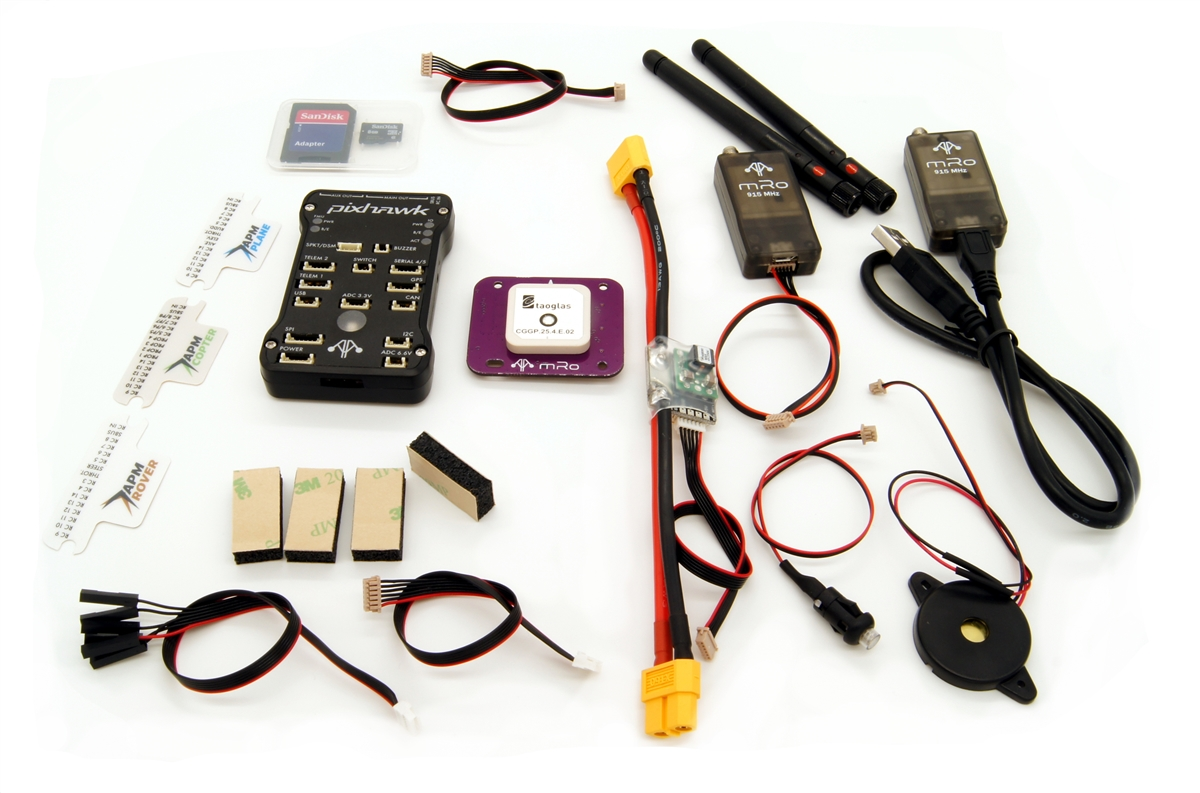
\includegraphics[width=0.8\linewidth]{figs/pixhawk.jpg}
  \caption{Pixhawk flight controller and most peripherals. Source: Mrobotics}
  \label{fig:pixhawk}
\end{figure}

\section{The GPS}
The used GPS is a U-Blox M8N GPS receiver, coupled with an external compass sensor. The external compass is important because the high currents flowing close the Pixhawk affect the readings of the internal compasses.
%
It supports concurrent reception of up to 3 GNSS (Global Navigation Satellite Systems), GPS, Galileo, GLONASS and BeiDou.

It's precision is around 3 m, occasionally getting lower than 1 m\cite{m8ntest}.

\begin{figure}[H]
\centering
  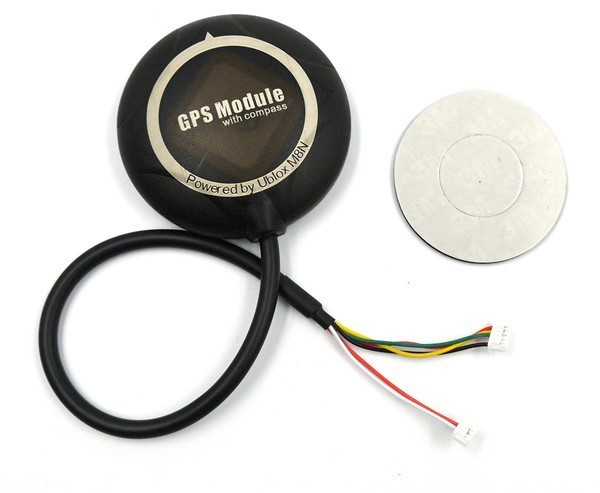
\includegraphics[width=0.8\linewidth]{figs/m8n.jpg}
  \caption{M8N GPS receiver and external compass. Source: cooltoyz.co.uk}
  \label{fig:m8n}
\end{figure}


\section{The Telemetry}

The telemetry system provides a serial (UART) connection to the aircraft, via a radio system.
%
The one used can be seen on the top right corner of Figure \ref{fig:pixhawk} and is a 900Mhz radio modem.
%
The telemetry allows real-time reading of parameters and attitude, as well as writing them for setup and tuning.

\section{The Radio Control System}

The used Radio System is a 2.4Ghz radio by Turnigy, the Turnigy 9x.
%
This radio uses fast frequency hopping to avoid interference, and has a reported range of up to 3 km \cite{range9x}.
%
The radio was modded\cite{t9xmod} and the firmware was replaced by the open-source OpenTX \cite{opentx}, which provides much more flexibility to the system, as custom mixes, switches, automatic functions, periodic functions, and telemetry capabilities.

\begin{figure}[H]
\centering
  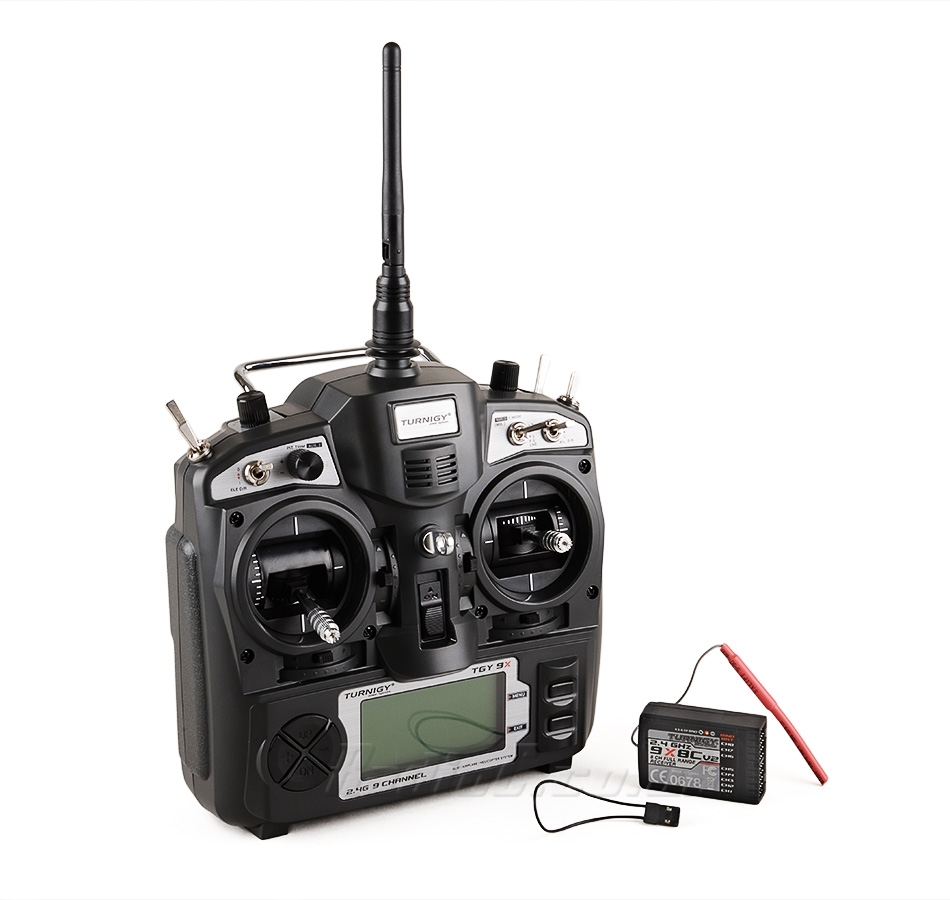
\includegraphics[width=0.8\linewidth]{figs/t9x.jpg}
  \caption{The Turnigy 9X Radio System. Source: radioc.co.uk}
  \label{fig:t9x}
\end{figure}


%%%%%%%%%%%%%%%%%%%